\documentclass{article}
\usepackage{graphicx}
\usepackage{multicol}
\usepackage[margin=0.5in]{geometry}
\begin{document}
\title{Matching Trig Graphs C}
\maketitle
\noindent
Write the name of the graph that matches the given equation. Use Graph Sheet
A and your knowledge of graph translations.
\begin{multicols}{2}
\begin{enumerate}
	\item $y=\tan(x+\frac{\pi}{3})$ \hspace{1cm} \rule{5cm}{0.5pt}
	\item $y=\tan(x-\frac{\pi}{3})$ \hspace{1cm} \rule{5cm}{0.5pt}
	\item $y=\tan(x-\frac{2\pi}{3})$ \hspace{1cm} \rule{5cm}{0.5pt}
	\item $y=\tan(x+\frac{7\pi}{4})$ \hspace{1cm} \rule{5cm}{0.5pt}
	\item $y=\sin (2(x-\frac{\pi}{3})) $ \hspace{1cm} \rule{5cm}{0.5pt}
	\item $y=\cos (2(x-\frac{\pi}{3}))$ \hspace{1cm} \rule{5cm}{0.5pt}
\end{enumerate}

\noindent
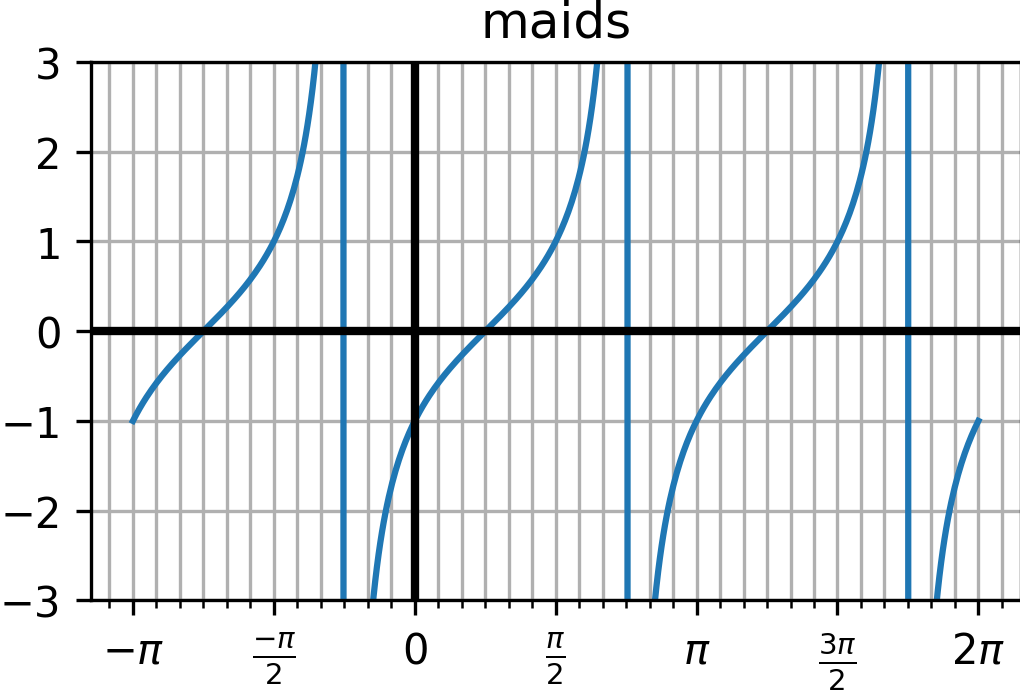
\includegraphics[width=3in]{maids.png} \\
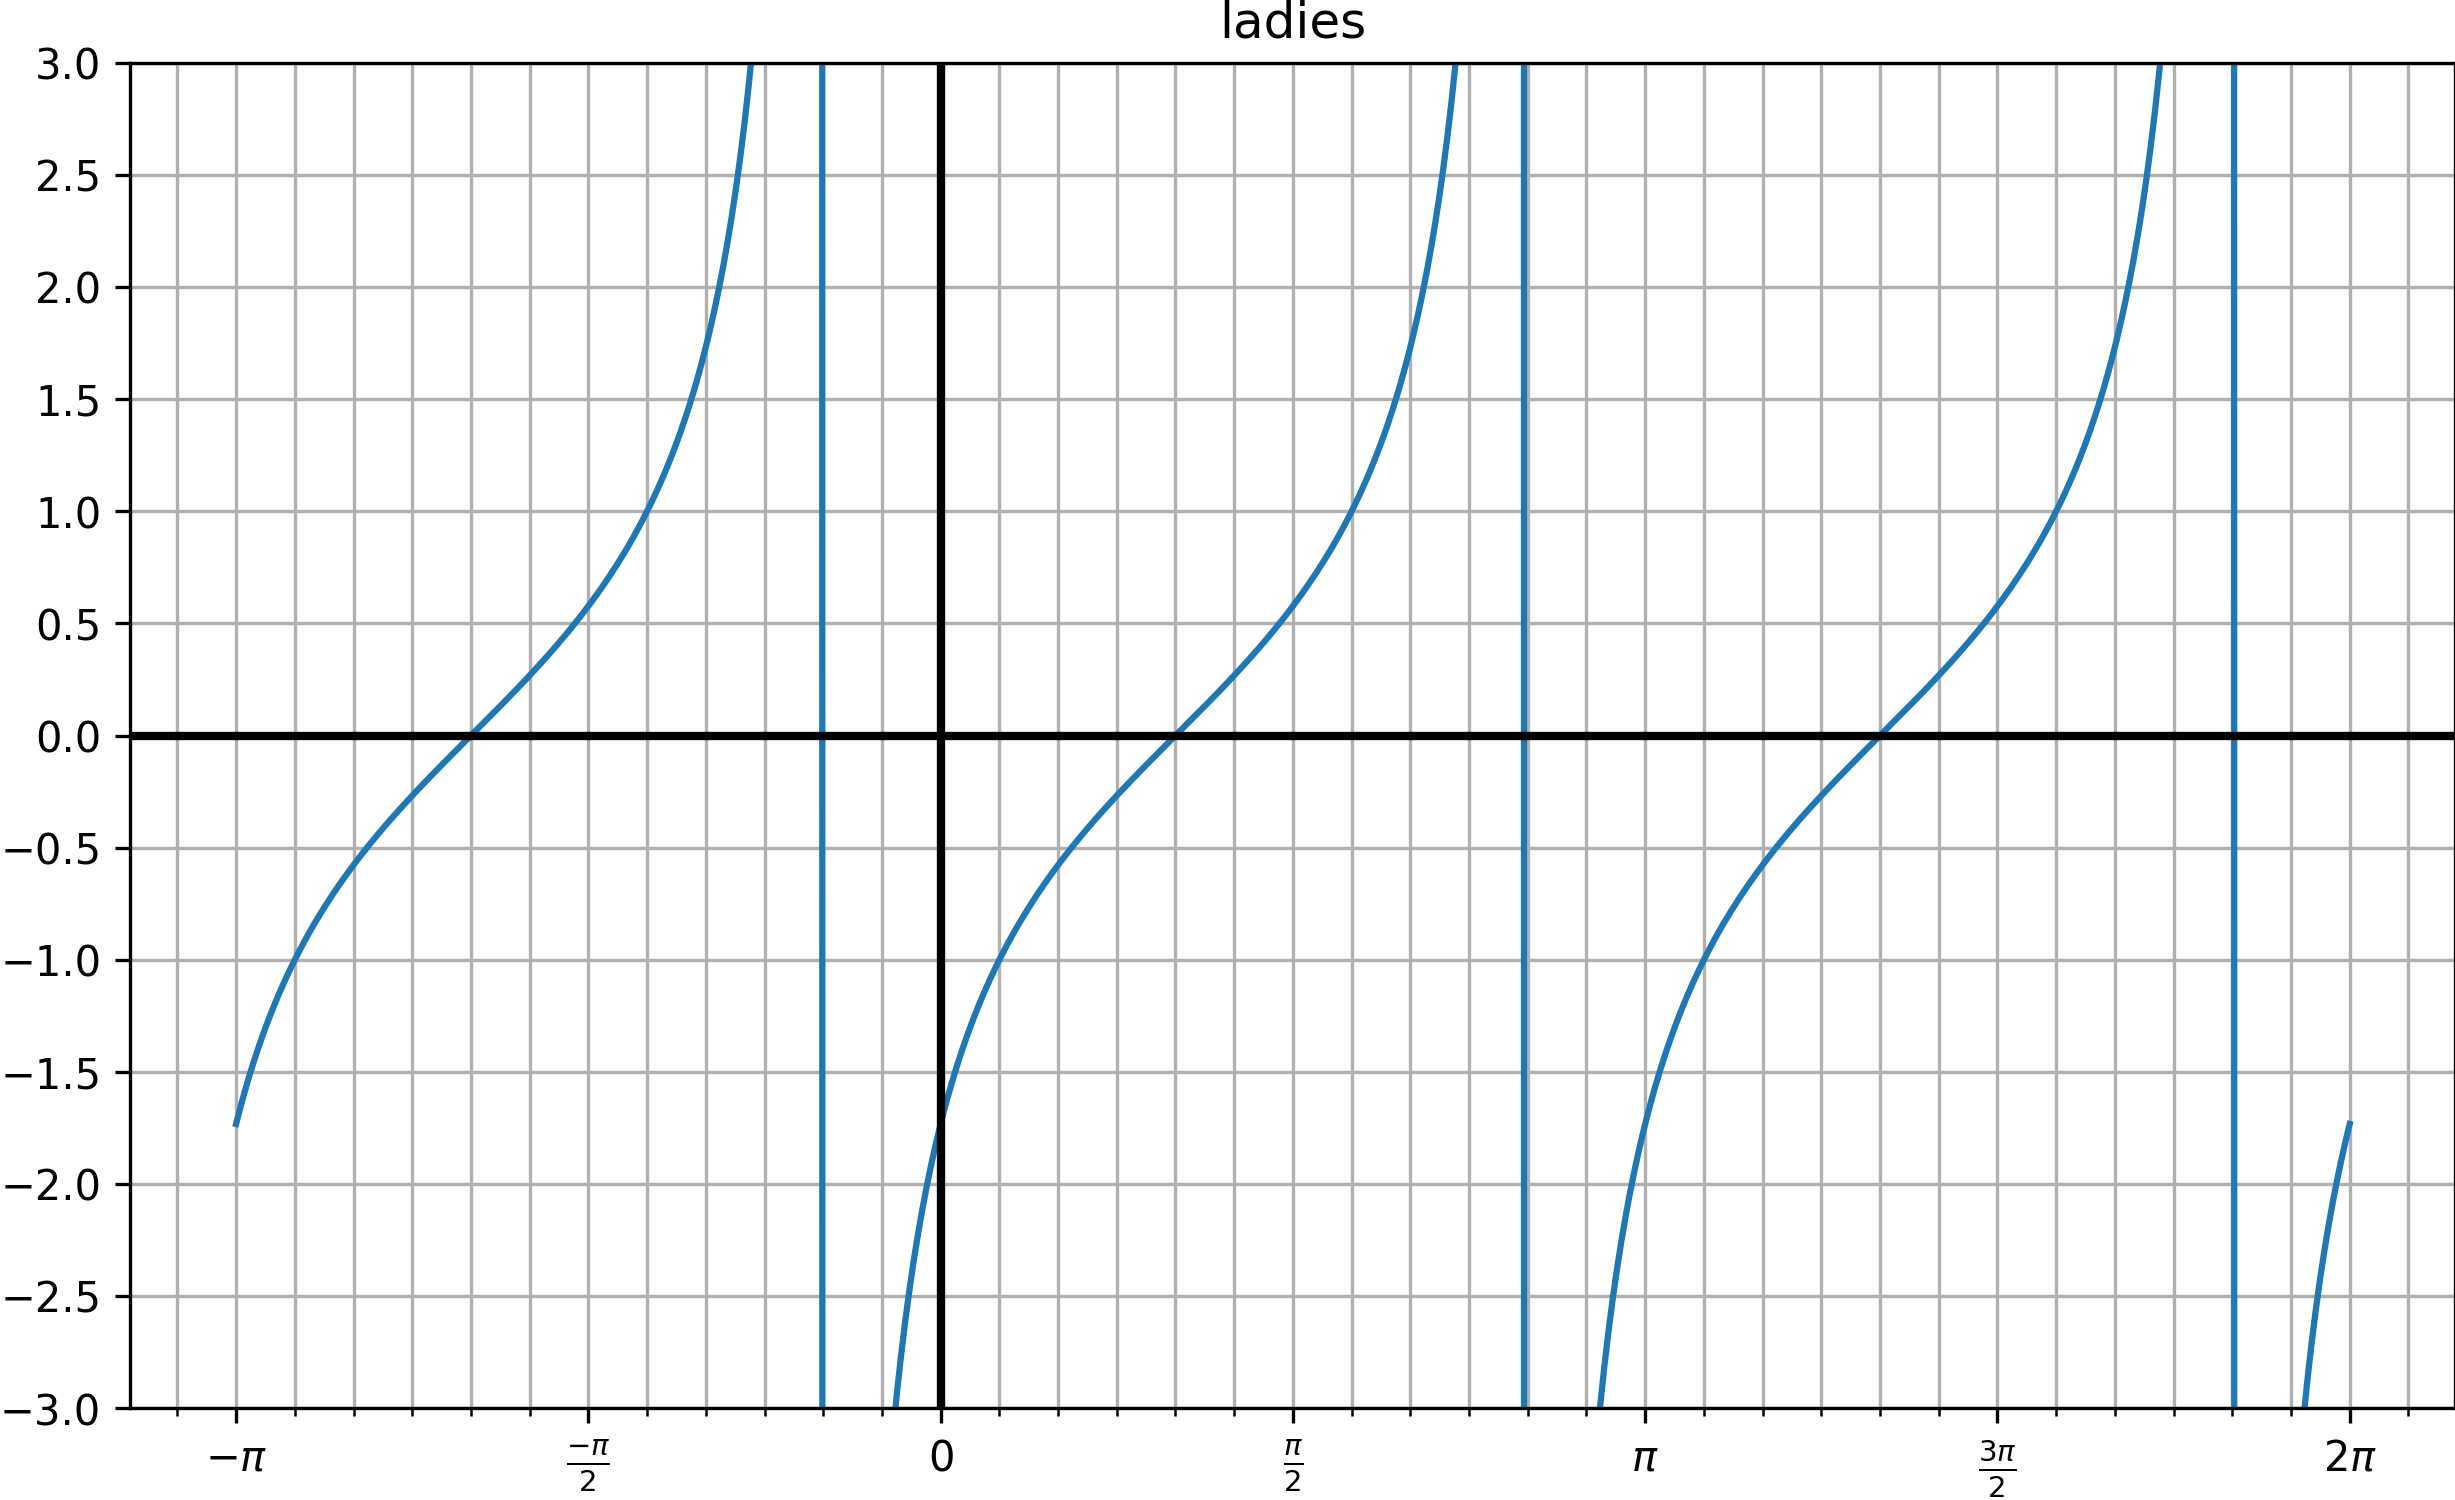
\includegraphics[width=3in]{ladies.png} \\
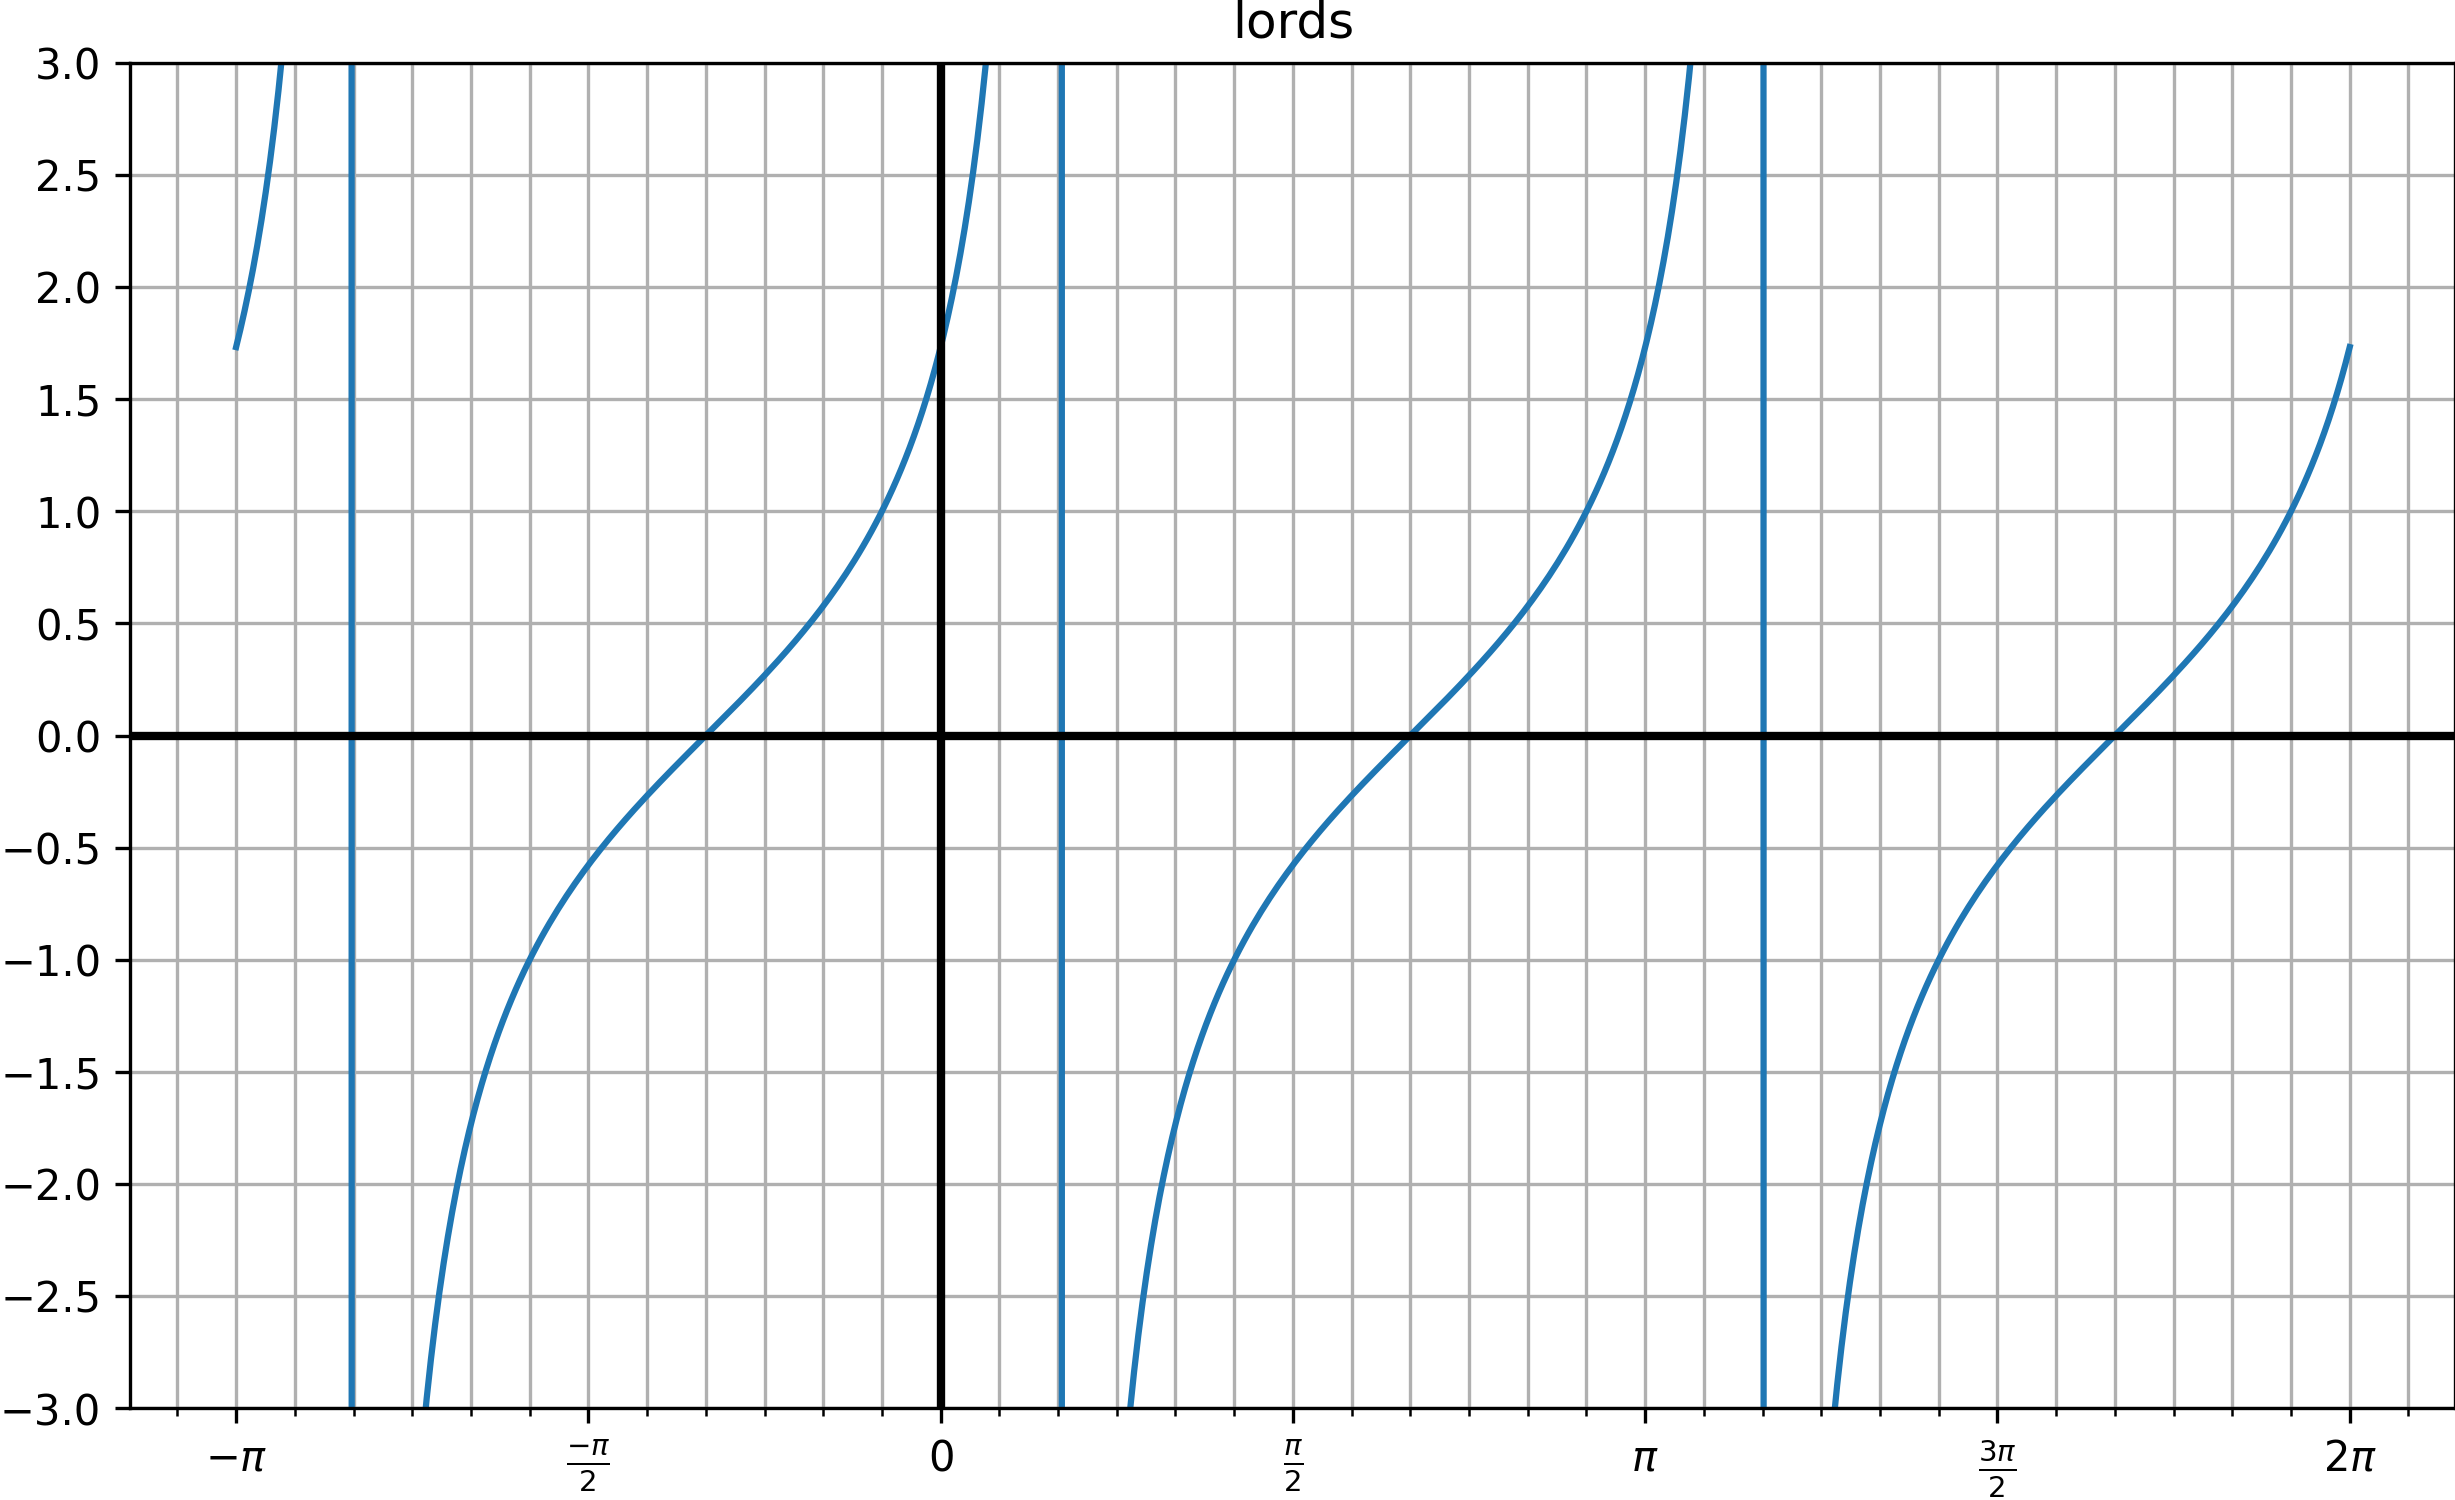
\includegraphics[width=3in]{lords.png} \\
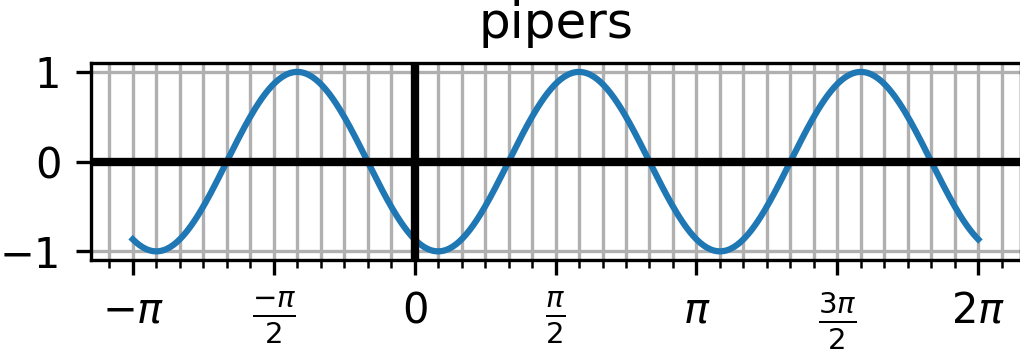
\includegraphics[width=3in]{pipers.png} \\
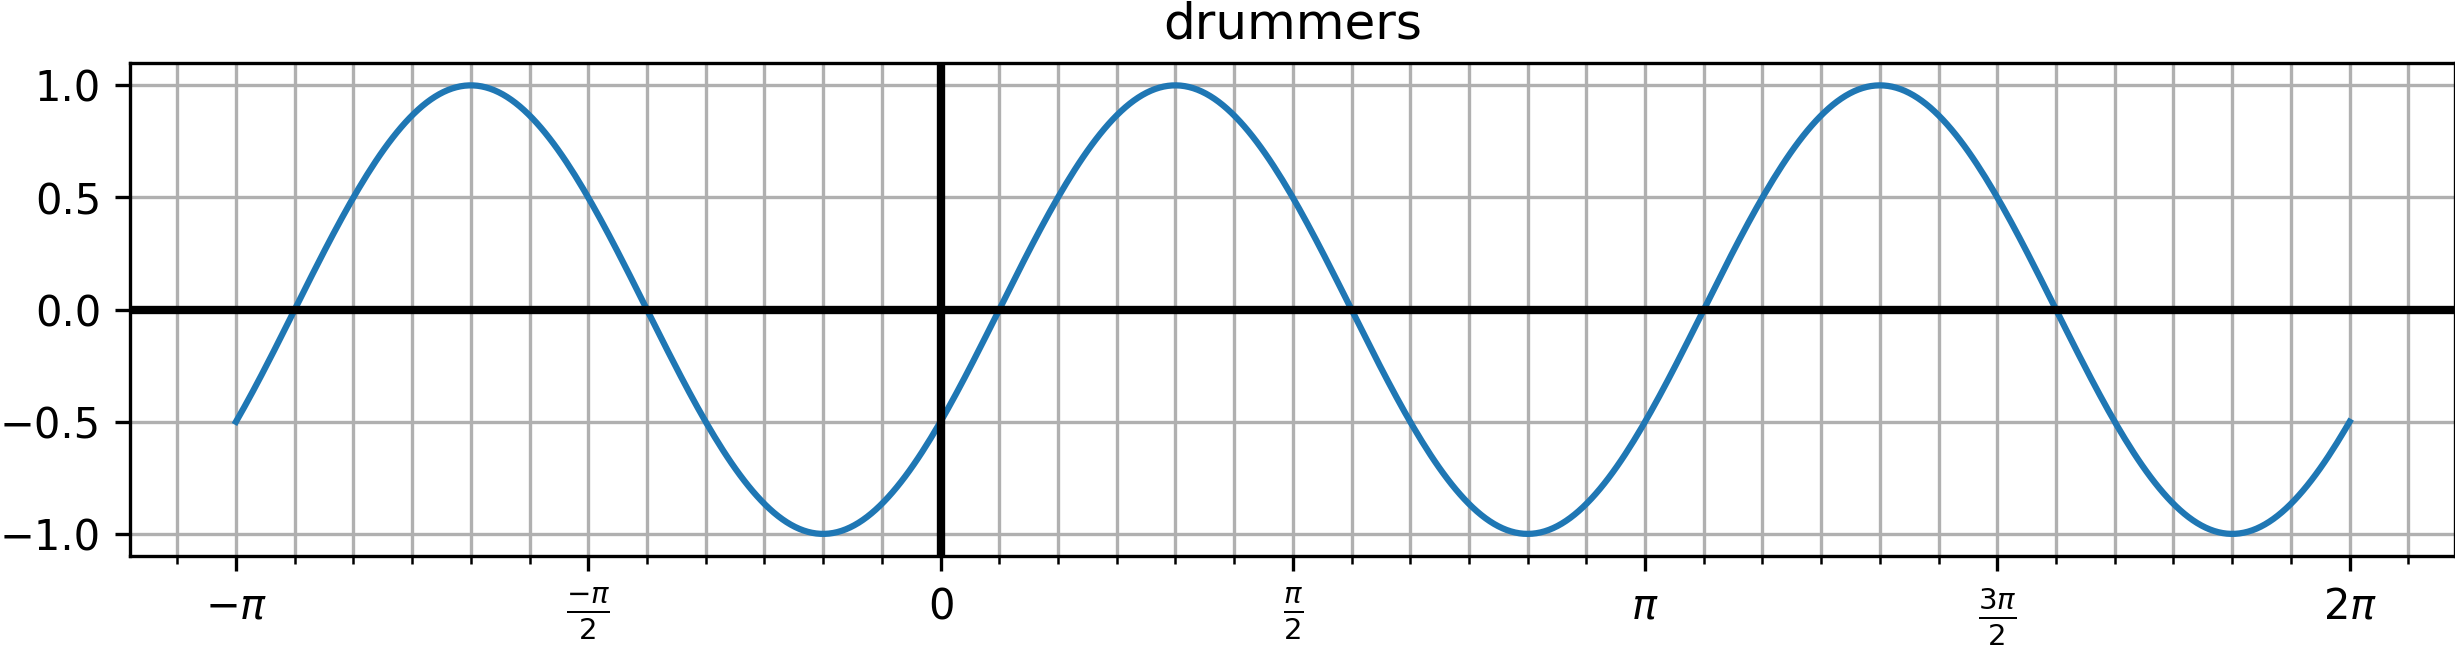
\includegraphics[width=3in]{drummers.png} \\
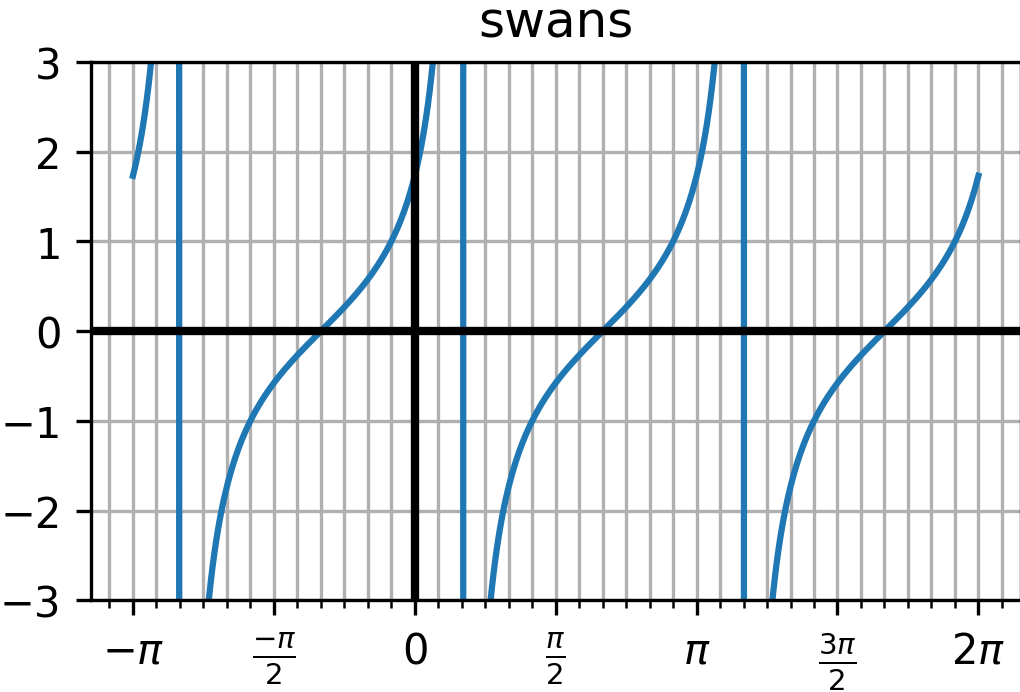
\includegraphics[width=3in]{swans.png}
\end{multicols}
\end{document}
